\documentclass[12pt]{article} % Default font size is 12pt, it can be changed here
\usepackage[utf8]{inputenc}
\usepackage{geometry} % Required to change the page size to A4
\geometry{a4paper} % Set the page size to be A4 as opposed to the default US Letter
\usepackage{listings}
\usepackage{parskip}
\usepackage[table]{xcolor}
\usepackage{float}
\usepackage{graphicx} % Required for including pictures
\usepackage{hyperref}
\usepackage{float} % Allows putting an [H] in \begin{figure} to specify the exact location of the figure
\usepackage{cite}
\usepackage{fancyhdr}
\usepackage{lscape}
\usepackage{eurofont}
\usepackage{wrapfig}
\usepackage{booktabs,colortbl, array}
\usepackage{pgfplotstable}
\usepackage{siunitx}

\linespread{1.2} % Line spacing

%\setlength{\parindent}{15pt}
%\setlength\parindent{0pt} % Uncomment to remove all indentation from paragraphs

\graphicspath{{../add/}} % Specifies the directory where pictures are stored
\pgfplotsset{compat=1.8}

\pagestyle{fancy}
\lhead{Repositorio de árboles genealógicos en BD NoSQL}
\rhead{Daniel Albarral Nuñez}
\cfoot{\thepage}
\renewcommand{\headrulewidth}{0.4pt}
\renewcommand{\footrulewidth}{0.4pt}
\begin{document}

\begin{titlepage}

\newcommand{\HRule}{\rule{\linewidth}{0.5mm}} % Defines a new command for the horizontal lines, change thickness here

\center % Center everything on the page
 
%----------------------------------------------------------------------------------------
%	HEADING SECTIONS
%----------------------------------------------------------------------------------------

\textsc{\LARGE Universidad Politécnica de Cataluña}\\[1.5cm] % Name of your university/college
\textsc{\Large Facultad de Informática de Barcelona}\\[0.5cm] % Major heading such as course name
\textsc{\large Ingeniería de software}\\[0.5cm] % Minor heading such as course 

%----------------------------------------------------------------------------------------
%	TITLE SECTION
%----------------------------------------------------------------------------------------

\HRule \\[0.4cm]
{ \huge \bfseries Repositorio de árboles genealógicos en BD NoSQL}\\[0.4cm] % Title of your document
\HRule \\[1.5cm]
 
%----------------------------------------------------------------------------------------
%	AUTHOR SECTION
%----------------------------------------------------------------------------------------

\begin{minipage}{0.4\textwidth}
\begin{flushleft} \large
\emph{Author:}\\
Daniel \textsc{Albarral Nuñez} % Your name
\end{flushleft}
\end{minipage}
~
\begin{minipage}{0.4\textwidth}
\begin{flushright} \large
\emph{Supervisor:} \\
Enric \textsc{Mayol} % Supervisor's Name
\end{flushright}
\end{minipage}\\[4cm]

% If you don't want a supervisor, uncomment the two lines below and remove the section above
%\Large \emph{Author:}\\
%John \textsc{Smith}\\[3cm] % Your name

%----------------------------------------------------------------------------------------
%	DATE SECTION
%----------------------------------------------------------------------------------------

{\large Q1 - 2015-2016}\\[2cm] % Date, change the \today to a set date if you want to be precise

%----------------------------------------------------------------------------------------
%	LOGO SECTION
%----------------------------------------------------------------------------------------


\includegraphics[scale=0.7]{add/logo_upc.png}\\[1cm] % Include a department/university logo - this will require the graphicx package
 
%----------------------------------------------------------------------------------------

\vfill % Fill the rest of the page with whitespace

\end{titlepage}

%----------------------------------------------------------------------------------------
%   TABLE OF CONTENTS
%----------------------------------------------------------------------------------------

\tableofcontents % Include a table of contents

\newpage % Begins the essay on a new page instead of on the same page as the table of contents 

\section{Planificación temporal}
La siguiente planificación económica tiene en cuenta los siguientes puntos:
\begin{itemize}
\item[•]El proyecto no esta orientado a dar rentabilidad económica.
\item[•]Todas las tareas se asignaran a la misma persona, el sueldo se supondrá según el rol que asuma en cada momento. 
\end{itemize}

\subsection{Identificación y estimación de costes}
\subsubsection{Costes de personal}
A pesar que el proyecto solo sera desarrollado por una única persona, durante el transcurso del proyecto asumirá diferente roles. Los costes de personal se estimaran calculando la carga de trabajo que tendrá que asumir cada rol, se establecerá el coste por hora a cada rol.

Ateniéndonos a la planificación temporal:
\begin{itemize}
\item La parte que corresponde a planificación, que va del día 09/14/2015 al 11/14/15, sera asignada al jefe del proyecto.
\item La primera fase de desarrollo, donde se configura el entorno de trabajo, que se comprende del 11/15/15 al 12/12/15, se asignara al de técnico de sistemas.
\newpage
\item Durante las siguientes fases del desarrollo, del 12/12/15 al 08/14/16, la carga de trabajo se distribuirá entre todos los roles. Estas fases se comprenden entre el 12/12/15 y el 05/14/16.
\begin{description}
\item[Jefe del proyecto] 5\%
\item[Programador] 70\%
\item[Sistemas] 10\%
\item[Tester] 15\%
\end{description}
\item La ultima fase donde se preparara la presentación del proyecto estará asignada al jefe del proyecto, del 05/15/16 al 06/14/16.
\end{itemize}
Contando una dedicación media de tres horas al día:


\setlength{\arrayrulewidth}{1mm}
\setlength{\tabcolsep}{12pt}
\renewcommand{\arraystretch}{2.5}
{\rowcolors{3}{green!80!yellow!50}{green!70!yellow!40}
\begin{tabular}{ |p{2cm}|p{2cm}|p{2cm}|p{2cm}|}
\hline
\multicolumn{4}{|c|}{Costes de personal} \\
\hline
ROL &Horas & \euro /hora &Coste total \\
\hline
Jefe del proyecto &274.8 &40 & 10992\\
Programador &431.2 &30 & 12936\\
Tester &92.4 &25 & 2310\\
Sistemas &169.6 &25 &4240\\
&&& 30478\\
\hline
\end{tabular}
}
\newpage

\subsubsection{Coste del espació de trabajo}

\begin{wrapfigure}{rh}{0.3\textwidth}
\begin{center}
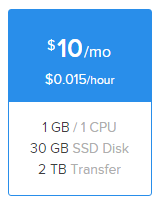
\includegraphics{add/do_server.PNG}
\caption{Precio y especificaciones del servidor}
\end{center}
\label{fig:do_server}
\end{wrapfigure}

Bajo el supuesto que se desarrollase el proyecto en un área de \textit{coworking}, concretamente coworking fontanella, el coste seria de 180\euros al mes, dado que el proyecto dura aproximadamente 9 mes, tal como podemos ver en la planificación temporal, implicaría un coste de 1620\euros.

\subsubsection{Coste del los servidores}
Durante la fase de \textit{deploy} se alquilaran servidores de digital ocean, el precio es de 10\euros al mes, dado que la fase de deploy dura un mes el coste sera de 10\euros .\linebreak

\newpage

\section{Sostenibilidad y compromiso social}
Cada una de las tres secciones siguientes están evaluadas sobre 10.
\subsection{Dimensión económica - 7}
El proyecto a desarrollar no busca la rentabilidad económica, por otro lado sus costes de desarrollo son muy bajos, siendo un proyecto muy viable económicamente. Si bien, en el caso de querer comercializar el software, como hemos podido ver en el estado del arte, es difícil que en el tiempo de duración del proyecto con los recursos que se disponen dar una solución del nivel de las soluciones actuales.
\subsection{Dimensión social - 9}
Al ser un software en el que todo su código sera abierto y integrara varias tecnologías que actualmente siguen en desarrollo, podrá ayudar a varias comunidades de desarrolladores. Por otro lado un resultado final del proyecto podría ser interesante para diferentes sectores dedicados a la genealogía que busquen una solución abierta para guardar la información de la que disponen.
\subsection{Dimensión ambiental - 6}
El proyecto tiene un mínimo impacto medio ambiental, no se espera que mediante el uso del software se ahorre ningún recurso material, pero el coste de mantenimiento y creación no implica consumir recursos materiales.




\end{document}



